\section{What is isomorphic to a qubit?}
\label{sec:math}
Fix the ordered orthonormal computational basis and write $\B=\{0,1\}$. Give $\C^{\B^n}$ its counting inner product. Define
\begin{align}
 W_n:(\C^2)^{\otimes n}&\longrightarrow\C^{\B^n},&
 W_n(\psi)(b)&=\langle b|\psi\rangle,&
 W_n^{-1}(f)&=\sum_{b\in\B^n}f(b)\ket b . \label{eq:isometry}
\end{align}
Orthonormality proves $W_nW_n^{-1}f=f$ by evaluation at $b$. Completeness of the basis proves $W_n^{-1}W_n\psi=\psi$. Expanding the inner product proves $\langle W_n\phi,W_n\psi\rangle=\langle\phi,\psi\rangle$. Thus $W_n$ is an isometric isomorphism for every finite $n$. It restricts to the unit spheres and descends to a bijection on rays because it commutes with scalar multiplication. One qubit has precisely a normalized two-label amplitude function up to common phase. Distinct basis choices give unitarily related maps.

The same coordinate change acts on transformations by $\widetilde A=W_n A W_n^{-1}$ and on states by $\widetilde\rho=W_n\rho W_n^\dagger$. Matrix multiplication, adjoint, tensor product with the agreed label order, trace and positivity are preserved. In particular $\Tr(\widetilde E\widetilde\rho)=\Tr(E\rho)$. For a completely positive map $\Phi$, conjugation on its input and output transports any Kraus representation and preserves complete positivity. It carries the trace-preserving condition into itself. If an instrument produces a classical label, the correspondence acts separately on each subnormalized output and hence preserves both its probability and its posterior state. This proves finite-register equivalence of the ideal mathematical models for all states and operations, including those specified by arbitrary complex parameters. Finite executable source and floating-point evaluation are separate levels.

\subsection{Recursive wavefunctions, entanglement and existence claims}
For $s\in\B^n$ put $f_0(s)=f(0s)$ and $f_1(s)=f(1s)$. Evaluation at the first bit gives
\[
 \C^{\B^{n+1}}\simeq \C^{\B^n}\oplus\C^{\B^n},\qquad
 \|f\|^2=\|f_0\|^2+\|f_1\|^2 .
\]
Joining the slices assigns $f_b(s)$ to $bs$. Splitting a joined pair recovers both components, and joining a split function recovers every amplitude. Lean verifies these identities simultaneously for all $n$ and any coefficient type. They give an exact recursive sense in which the representation repeats at each level. Calling this a fractal is an interpretation. The statement requires neither a metric scaling law nor a noninteger fractal dimension. The same first wire has a pure local state precisely when the nonzero slices are proportional, or equivalently the bipartite pure state's Schmidt rank is one.

For the Bell state the two slices are $\ket0/\sqrt2$ and $\ket1/\sqrt2$. Their squared norms are the probabilities of measuring the prefix. Conditional on outcome $b$ the remaining state is $\ket b$. Discard that classical outcome and the remaining qubit is $I/2$. More directly, a hypothetical local pure state matching the $Z$ probabilities would have amplitudes of magnitude $1/\sqrt2$, and hence an off-diagonal density element of magnitude $1/2$. The actual local density has zero there. This is an experimental distinction visible in other bases. For the whole pair a pure wavefunction exists before measurement.

Subsets also have a precise interpretation. A subset $S$ of basis labels defines an event $P_S=\sum_{b\in S}\ket b\bra b$, with probability $\sum_{b\in S}|f(b)|^2$. Every subset of a fixed finite basis indeed has such an event. Rotated projectors describe other sharp events, and arbitrary effects allow unsharp tests. A two-dimensional logical subspace of a larger system can serve as a qubit once an encoding is specified. None of these constructions supplies a map that identifies all objects or all subsets of existence with pure states of one qubit. For example, a qutrit has three mutually orthogonal preparations, and an isometry to a single qubit would have to preserve three orthogonal vectors in dimension two.

\subsection{Mixed states as actual functions}
For a density matrix define $R_\rho(E)=\Tr(\rho E)$ for each effect $0\le E\le I$. The probabilities of $E_j=(I+\sigma_j)/2$, $j=x,y,z$, give $r_j=2R_\rho(E_j)-1$. The inverse is $\rho=(I+\mathbf r\cdot\boldsymbol\sigma)/2$. Positivity is equivalent to $|\mathbf r|\le1$, purity to $|\mathbf r|=1$. For $E=aI+\mathbf v\cdot\boldsymbol\sigma$ the admissibility conditions are $0\le a-|\mathbf v|$ and $a+|\mathbf v|\le1$. The response is $a+\mathbf v\cdot\mathbf r$. The physically admissible effect-response functions are affine and normalized, and the inverse shows injectivity. An unknown state need not be reconstructed in a single shot. Measurements sample the responses on separately prepared copies.

\begin{figure}[ht]
\centering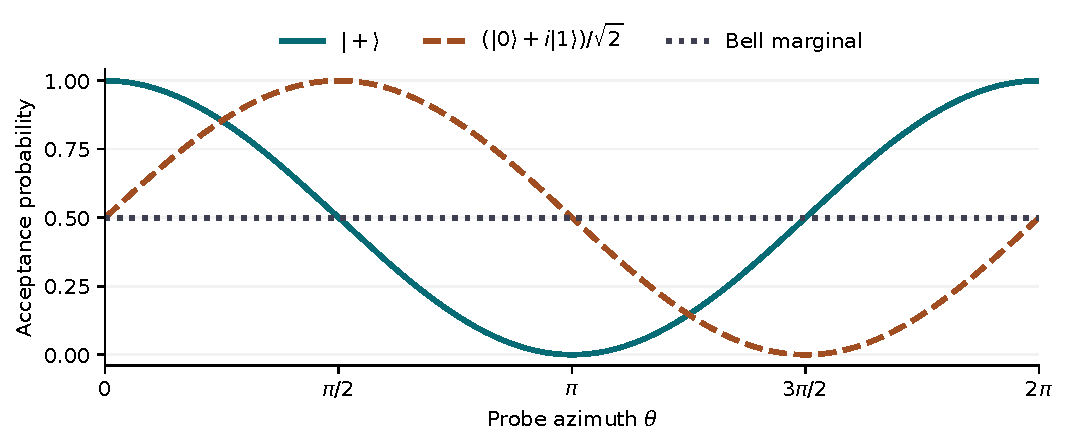
\includegraphics[width=.88\linewidth]{responses.pdf}
\caption{Born responses to an equatorial probe with azimuth $\theta$. The pure states $\ket{+}$ and $(\ket0+i\ket1)/\sqrt2$ and the reduced state of a Bell qubit all give computational probabilities $(1/2,1/2)$. Changing the probe distinguishes them. The constant line also follows by tracing out either wire of the simulated Bell state.}\label{fig:responses}
\end{figure}

A class in QAF names a collection of fields and methods. Its quantum interpretation depends on invariants and admissible operations. An amplitude class with two complex fields presents $\C^2$. Enforcing unit norm and identifying global phase gives pure qubit rays. A finite classical record type $X$ has a distinguishable encoding in the basis of $\ell^2(X)$. Deterministic classical transitions extend to channels on diagonal states. A permutation gives a unitary basis action. A many-to-one map needs an environment if implemented reversibly. A two-entry Boolean truth table has four possible classical values, so an orthogonal encoding of all tables needs two qubits. A class declaration with unrestricted arithmetic has no canonical one-qubit isomorphism.

\subsection{Five operations on functions}
Let $\mathcal A=\C^\B$. Addition, subtraction and multiplication mean pointwise arithmetic. Division $f/g$ has domain $\{(f,g):g(0)g(1)\ne0\}$ when a total two-label result is required. Composition $g\circ f$ requires the codomain of $f$ to match the domain of $g$. Two maps $\B\to\C$ therefore have no general ordinary composite. Precomposition by $h:\B\to\B$ is defined by $(f\circ h)(b)=f(h(b))$. Composition of amplitude \emph{kernels} means matrix composition $(LK)(y,x)=\sum_z L(y,z)K(z,x)$. These rules give three useful kinds of composition without coercing a complex amplitude into a wire label.

Function extensionality proves the ring laws by evaluation at each $b$. Addition and multiplication are commutative and associative, multiplication distributes over addition, and the pointwise constant functions are the respective identities. Subtraction satisfies $(f-g)+g=f$ and $f-f=0$. Wherever the quotient is defined, $(f/g)g=f$. Typed composition is associative with the corresponding identities. Neither subtraction nor division is associative in general. The Lean proofs use scalar-field laws as hypotheses. The example below executes all five operations and normalizes only at state preparation.
\inputminted[firstline=55,fontsize=\footnotesize]{qaf}{examples/prefix/algebra.qaf}
The result is $(i,1)/\sqrt2$. A zero denominator rejects evaluation. The zero function is perfectly meaningful in $\mathcal A$ and has no normalized ray. Arithmetic on representatives can also depend on phase choice: replacing $\ket0$ by $-\ket0$ leaves its ray invariant, while adding $\ket1$ then yields distinguishable rays. An operational superposition needs a phase reference and a preparation procedure. Normalizing a classical specification and evolving an unknown state by a deterministic physical channel are different interfaces. The typed preservation theorem in the archive quantifies over physical expressions whose preparations and transformations have supplied validity witnesses. It does not assert closure of all unrestricted classical expressions as pure qubits.

\section{Tensor rank, infinite width and the scope of universality}
\label{sec:infinite}
Let $H_A,H_B$ be separable complex Hilbert spaces. A unit vector in their completed Hilbert tensor product has a Schmidt expansion $\psi=\sum_{k\ge0}s_k u_k\otimes v_k$ with orthonormal families, $s_k\ge0$ and $\sum_k s_k^2=1$ \cite{schmidt,cleve}. Orthogonal projection onto the first $R$ terms leaves squared norm error $\delta_R=\sum_{k\ge R}s_k^2$. For the renormalized truncation $\psi_R$ one has $|\langle\psi,\psi_R\rangle|^2=1-\delta_R$. Its pure-state trace distance from $\psi$ is $\sqrt{\delta_R}$, which bounds the change in the probability of any effect. A specified fixed product basis also gives convergent square projections, even when it is different from the Schmidt basis. The Schmidt argument concerns a bipartition. For three or more factors a best approximation of fixed canonical tensor rank can fail to exist \cite{tensorrank}.

\textbf{Density theorem.} Choose a countable orthonormal basis of a separable $H$ and identify its coordinates with a subset of $\mathbb N^2$. For every unit vector $\psi$ and every $\epsilon>0$, there is a finite QAF \texttt{hilbert} program whose normalized state has Hilbert norm distance below $\epsilon$ after the fixed embedding. Indeed choose a finite projection whose omitted norm is below $\epsilon/4$. Approximate the retained complex coefficients by Gaussian rationals with total $\ell^2$ error below $\epsilon/4$. The resulting vector $v$ is given by a finite sum of QAF \texttt{basis} terms. The triangle inequality and $|1-\|v\||\le\|v-\psi\|$ give $\|v/\|v\|-\psi\|\le2\|v-\psi\|<\epsilon$, choosing the approximant nonzero. Finite-rank normalized density operators are similarly dense among density operators in trace norm by spectral truncation; rational pure approximants with approximated mixture weights give finite preparation ensembles. The pure-state theorem is an existence result. A procedure that selects a rank from data requires an effective tail bound.

There is an exact computational case with infinite Schmidt rank. Set
\[
 \ket{\psi_t}=\sqrt{1-t^2}\sum_{k=0}^{\infty}t^k\ket{k,k},\quad
 K(t,u)=|\langle\psi_t|\psi_u\rangle|^2
       ={(1-t^2)(1-u^2)\over(1-tu)^2}
\]
for rational $|t|,|u|<1$. The discarded mass beyond $R-1$ is $t^{2R}$. QAF also supports finite complex rational superpositions of individual basis vectors and two independently geometric product modes. Every cross term has a finite geometric-series formula for its projected inner product, and an absolutely convergent closed form at infinite rank. The evaluator computes exact rational fidelities and truncation masses. Projection can generate an ordinary QAF circuit for GPU execution. Here is a complete input.
\inputminted{qaf}{examples/prefix/hilbert.qaf}
The exact answers are $3^{-16}$, $24/25$ and $-64/225$. At rank eight the projected state's trace distance is $3^{-8}=1/6561$. This bounds the error of all effect probabilities, including ones absent from the listing. A finite cutoff alone would not give a uniform bound on expectations of an unbounded position, momentum or energy observable. Such a claim would require domain and moment estimates.

To see why the classifier has a quantum meaning, use rank-one density matrices as features in the real Hilbert space of self-adjoint Hilbert--Schmidt operators. Their inner product is $\Tr(\rho\sigma)=|\langle\psi|\phi\rangle|^2$ for pure states. This kernel is positive semidefinite since each finite Gram quadratic form is a squared Hilbert--Schmidt norm. For two training features $\rho_+$ and $\rho_-$ of unit norm and opposite labels, the minimum-norm hard-margin separator with intercept zero is $w=(\rho_+-\rho_-)/(1-\Tr(\rho_+\rho_-))$. Both constraints bind. Cauchy--Schwarz applied to their difference proves minimality. Here the training states use $t=0$ and $t=1/2$. The score at $t=1/3$ is $4(8/9-24/25)$. Its change under truncation is bounded by $\|w\|_2\sqrt{2\delta_R}$. This explicit kernel machine is an observable-derived classifier. An arbitrary learned decision score requires rescaling or calibration before interpretation as a probability.

Cortes and Vapnik's SVM optimizes a margin in a chosen feature space \cite{svm}. Chen and colleagues prove that an infinitely wide network with a suitable limiting neural tangent kernel and regularized hinge loss has the same output dynamics as a soft-margin SVM with that kernel, given matching initial outputs and the paper's smoothness and scaling conditions \cite{chen,ntk}. Their network can have nonlinear hidden layers. A predictor linear in feature coordinates can be nonlinear in its original input. A different theorem gives a hard-margin limiting direction for training certain fully connected linear networks on separable data, subject to convergence assumptions \cite{gunasekar}. The two-support classifier above uses the specified quantum fidelity kernel. Equating it to the tangent kernel of any particular deep architecture would require a derivation for that architecture.

Universal approximation likewise needs a function class and error norm. Cybenko proves uniform density on a compact cube for a family with nonlinear sigmoidal activation \cite{cybenko}. Linear layers alone compose to an affine map on their input. A linear model with an infinite feature map can nevertheless have a rich function class. A nonlinear classical representation of amplitudes is consistent with the linear evolution of the physical ket. The QAF density theorem gives a direct universality statement in the norm relevant to a quantum state, including square-integrable states lacking continuous representatives.

The quantifiers determine how far the result extends. Every separable pure state has approximants at every positive tolerance. Exact execution by a finite program has a short obstruction even for one qubit: take $\sqrt{1-p}\ket0+\sqrt p\ket1$ for $p\in[0,1]$. Measuring $\ket1\bra1$ recovers $p$ as the exact probability. There are uncountably many choices and countably many finite program texts over the language's alphabet. Supplying an arbitrary real-valued oracle as an extra input changes that statement and specifies where the missing information resides. Complete mathematical representation relative to an abstract amplitude function, approximation by executable preparations, and exact computation of particular observables therefore have different proofs.
